\documentclass{article}

\usepackage{qtree}
\usepackage{graphicx}

\begin{document}
\title{Homework 10}
\date{}
\maketitle

% 1. Given an LLRB, is there exactly one corresponding 2-3 tree? Given a 2-3 tree, is the exactly one corresponding LLRB?
% 2. Draw a 2-3 tree with all 3 nodes. Why is the height log3(N)?
% 3. How many compares does it take in the worst case to decide whether to take the left, middle, or right link from a 3 node?
% 4. Fall 2010 Midterm Question 4, Fall 2011 Midterm Question 6, Spring 2012 Midterm Question 5, Spring 2013 Midterm Question 2, Fall 2008 Midterm Question 6, Fall 2009 Midterm Question 4,

\paragraph{\Large 1. Study Guide Question}\mbox{}\\
Given an LLRB, is there exactly one corresponding 2-3 tree? Given a 2-3 tree, is the exactly one corresponding LLRB?\\

2-3 trees and LLRBs have an exact 1-1 correspondence. For any 2-3 tree there is exactly one LLRB tree and vice versa.

\paragraph{\Large 2. Study Guide Question}\mbox{}\\
Draw a 2-3 tree with all 3 nodes. Why is the height log3(N)?\\

\Tree [ .{1 2} [ .{3 4} {9 10} {11 12} {13 14} ] [ .{5 6} {15 16} {17 18} {19 20} ] [ .{7 8} {21 22} {23 24} {25 26} ] ]\\
Each node of the tree has 3 children, leading to a height of $\left \lceil{\log_3{N}}\right \rceil$

\paragraph{\Large 3. Study Guide Question}\mbox{}\\
How many compares does it take in the worst case to decide whether to take the left, middle, or right link from a 3 node?\\

It takes 2 compares in the worst case as eliminating 2 of the three children is all that is necessary to decide to take the third.

\paragraph{\Large 4. One of the following: Fall 2010 Midterm Question 4, Fall 2011 Midterm Question 6, Spring 2012 Midterm Question 5, Spring 2013 Midterm Question 2, Fall 2008 Midterm Question 6, Fall 2009 Midterm Question 4}\mbox{}\\
Consider the following left-leaning red-black BST.\\
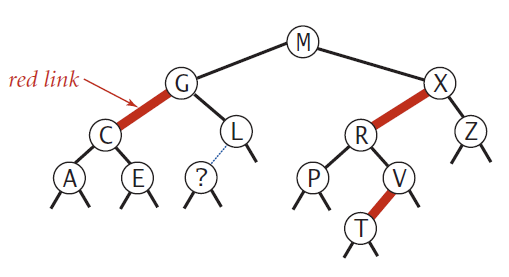
\includegraphics[width=\linewidth]{RBTree.PNG}\\

\begin{enumerate}
\renewcommand{\theenumi}{\Alph{enumi}}
	\item Which one or more of the keys below could be in the node labeled with a question mark?\\
	A B C D E F G H I J K L M N O P Q R S T U V W X Y Z\\\\
	H, I, J, and K
	\item What is the color of the link from the node labeled with a question mark to its parent?\\\\
	Red
	\item Add the key U and draw the resulting left-leaning red-black BST.\\
	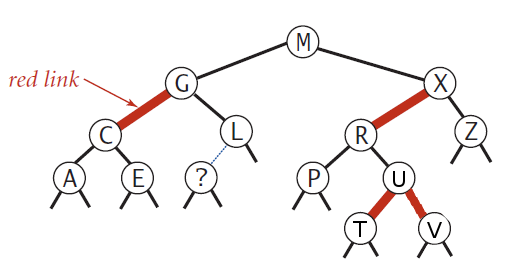
\includegraphics[width=\linewidth]{RBTree2.png}\\

\end{enumerate}

\end{document}